\documentclass[11pt,a4j]{jsarticle}

\usepackage{float,array,booktabs,here}
\usepackage{amsmath}
\usepackage[dvipdfmx]{graphicx}
\usepackage[top=15truemm,bottom=20truemm,left=20truemm,right=20truemm]{geometry}
\usepackage{url}
\usepackage{listings, jlisting}

\lstset{language=c,
  frame=single,
  stepnumber=1,
  numbersep=2pt,
  tabsize=2,
  basicstyle=\verysmall\ttfamily,
  stringstyle=\small\texttt,
  commentstyle=\slshape,
  captionpos=b,
  columns=[l]{fullflexible}
}

\makeatletter
\newcommand{\figcaption}[1]{\def\@captype{figure}\caption{#1}}
\newcommand{\tblcaption}[1]{\def\@captype{table}\caption{#1}}
\makeatother

\newcommand{\Maru}[1]{\ooalign{
\ifnum#1<10 \hfil\resizebox{.9\width}{.85\height}{#1}\hfil
\else
\hfil\resizebox{.6\width}{.8\height}{#1}\hfil
\fi
\crcr
\raise.1ex\hbox{$\bigcirc$}}}



\begin{document}

\input{title}

\section{DB設計}

\begin{figure}[H]
  \centering
  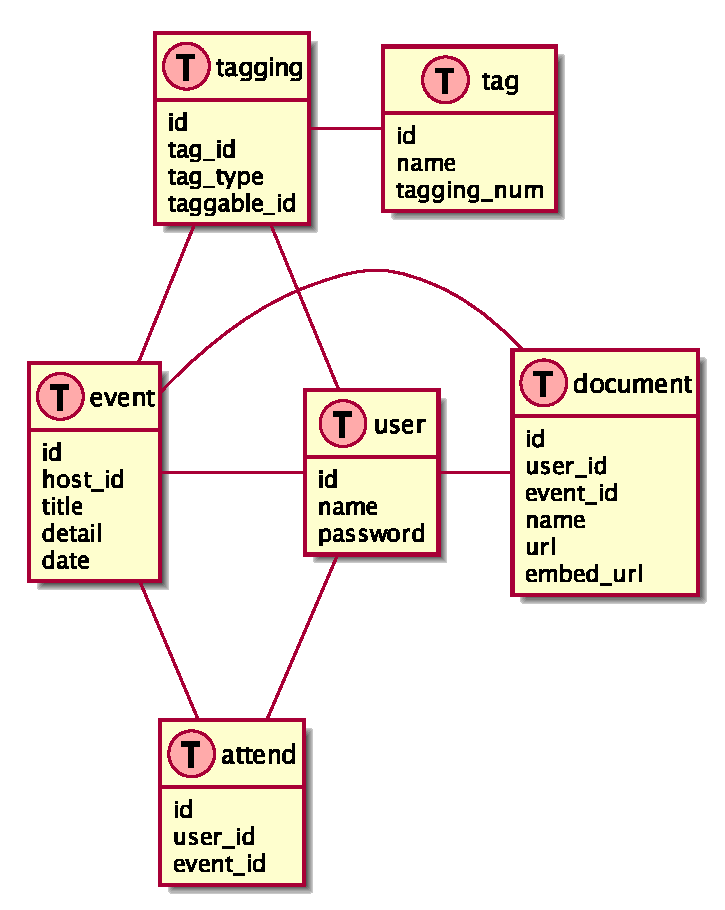
\includegraphics[scale=0.7]{img/data.eps}
  \figcaption{DB設計}
  \label{fig:db}
\end{figure}


\section{機能紹介}

\subsection{機能1 ユーザー登録、ログイン、パスワード変更}

まずは、ユーザー登録という、アプリケーションを使用する上で必須となる項目の実装を行なった
ユーザー登録において、ユーザーネームとパスワードにバリデーションを設けることは行わなかったため、クロスサイトスプリクティングの
脆弱性を生んでしまっていた。簡単に判定を行えたので、実装すべき点であった。

\subsection{機能2 イベント登録、編集、消去}

本アプリのメイン機能であるイベントの管理部分のシステムである。

イベントの登録では、クロスサイトスプリクティングの対策は講じてある。
内容としては、本文や、タイトルなどの箇所ではhtmlセーフな形に中身を変えて表示を行うというものである。

イベントの登録時には、イベント情報とともにタグを付与することを可能とした。
タグの管理はtag,taggingの二つのテーブルを用いて管理している。
タグはユーザーにつけることも想定していたため、図\ref{fig:db}のような設計となっている。

tagテーブルには、tagging\_numというタグの付与されている数を数えるカラムが存在するが、
タグ一覧などを表示する際に、全てのタグに対してtaggingされている数を数えるのと、taggingの更新のたびに、
tagのデータベースに更新をかけるののコストを考えた際により良いと思えるtagging\_numカラムの作成を行うこととした。

\subsection{機能3 スライドの登録、消去}

技術系イベントでは、資料がイベント中に使われることがよくある。
その中で、イベント終了後などに、資料を主催者が参加者達に対して簡単に開示できる仕組みは必要だと考えられる。
そこで、イベントごとに資料ページを用意して資料の追加を簡単に行えるようにした。

また、資料の追加では、slideshareのリンクを貼るだけで、そのページからスクレイピングを行なって適切な
iframeのリンクを生成するようにした。

他のスライドサイトとして、googleslide, speakerdeck, preziなどがあるが同様にスクレイピングを行いながら
色々なスライドを追加できるようにすることも簡単に実装できるであろう。

\section{その他工夫した点}

今回はフレームワークなどを用いないPHPでの開発であったため、なるべく楽をできるよう
またRESTfulなURLとなるように工夫をした。
具体的にはmodelごとにフォルダとして、/{model\_name}/action.phpというアドレスとなることを目指した。
こうすることで、コーディングの際にも、目的のファイルを簡単に探すことが可能となり、効率的なコーディングが行えた。

また、アプリのルートとなるURLなどを、全てのファイルで書き込むのは手間であったため、helperとなる関数を定義していった。
具体的には、application\_helperを一つ、helperをmodelの数だけ用意するということを行なった。
この中でglobalな変数を用意することで、効率的にファイルの連携を行うことが可能であった。

また、他にクエリの定義する変数の名前といった、変数の命名規則に気を使った。


\section{感想}

最初から、上述したコードの設計をしっかりと行えばよかったというのが一番の感想です。
命名規則など最初から気をつけていれば、もう少し色々できたなと。。

後は、viewの作成が大変でした。今回は外部から持ってきたcssをうまく利用しては行きましたが、
cssを書き換える、書き足すところも多々あり、ほとんどの時間をviewに咲いてしまったので
ロジックを詰めきれていないのが勿体無かったです。




\end{document}
